
%+
% SECTION:
%    supernovacosmology.tex
%
% CHAPTER:
%    cosmology.tex
%
% ELEVATOR PITCH:
%    SNIa cosmology, approach to evaluating dependence of science on cadence
%
%-
% ====================================================================

\section{Supernova Cosmology and Physics}
\def\secname{supernovae}\label{sec:\secname}

\credit{jhrlsst},
\credit{MichelleLochner},
\credit{rbiswas4},
\credit{sethdigel}.

This section is concerned with the detection and characterization of
supernovae (SNe) over time with LSST and their various scientific
applications. A crucial application is the use of supernovae type
Ia (SNIa) and potentially some core-collapse SN (like type IIP) to trace
the recent expansion history of the universe, and confront models of the
physics driving the late time accelerated expansion of the universe.

LSST will improve on past surveys by observing a substantial number of well-characterized 
supernovae, at high redshift. This large sample is not necessarily tied to the large area of LSST 
and can rather be obtained from a relatively small spatio-temporal region with larger numbers of 
well-measured light curves.

On the other hand, the WFD aspect will make the LSST survey 
the first to scan a very large area of the entire Southern sky for
SNe. SNe that are detected and well characterized by LSST can trace
large scale structure in a novel way, and include estimates of radial distances, as 
well as
their own redshift estimates that may be used in conjunction with host
galaxy redshift information. Due to these properties, they can probe the
isotropy of the late time universe.    

In addition, this large sample will
enable further sharpening of our understanding of the properties of the
SN population of different types (see \autoref{sec:SNtransients}). This last point is extremely 
important
for SN cosmology goals as the success of SNIa cosmology has always been
based on the empirical model that intrinsic peak brightnesses are
related to the certain observable characteristics of SNe.  The WFD SNIa
sample will dramatically increase the size of the sample available to
train such an empirical model, as well as understand the probability of
deviations and scatter from this model. Aside from issues like
calibration which need to be addressed separately, a larger sample of
such well measured SNe is probably the only way to address `systematics'
due to deviations from the empirical model. The anticipated sample can
be thought of as consisting of two components:  the low-redshift sample
which is more likely to be complete, and the higher-redshift sample that
will be able to constrain evolution.

% --------------------------------------------------------------------

\subsection{Target measurements and discoveries}
\label{sec:\secname:targets}

SNe of different types are visible over time scales of about a few
weeks (e.g., type Ia) to nearly a year (type IIP).  During the full
ten-year survey, LSST will scan the entire southern sky repeatedly with
a WFD cadence, and certain specific locations of the sky called the Deep
Drilling Fields (DDF) with special enhanced cadence.

This spatio-temporal window should contain millions
of SNe, that will have apparent magnitudes brighter than the single
exposure limiting magnitude of LSST. However, the actual sequence of
observations by LSST, defined by the series of field pointing as a
function of time in filter bands (along with weather conditions), will
determine the extent to which each SN can be detected and characterized
well.  Characterization of the SNe is at the core of a number of science
programs that use them as bright, abundant objects with empirically
determined intrinsic brightnesses. 

For LSST, this goal entails: 
\begin{enumerate}
\renewcommand{\theenumi}{\alph{enumi}}
\item The detection of SNe \label{it:detection}
\item Photometric classification \label{it:typing}
\item Estimation of photometric redshifts of SNe (or identifying host galaxies and obtaining their
redshifts from photometry or follow-up spectroscopy) \label{it:redshift}
\item Estimation of intrinsic brightnesses of the SNe \label{it:mu}
\item Constructing a Hubble diagram with this data for cosmological inference \label{it:cosmology}
\end{enumerate}

The efficacy
of photometric typing, redshifts and estimation of intrinsic brightnesses
are all dependent on the amount of information available in the observed
light curves of SNe. While these steps are not necessarily independent, it
is useful to think of the requirements on some of these steps separately;
it is not unlikely  that combinations of some of the steps would still be
affected by similar requirements. Ultimately, any cosmological figure of merit (the $w_0-w_a$ 
figure of merit described in \citet{Albrecht2006} for example) will depend on intermediate metrics 
describing each of these steps in turn. Here we focus on steps \ref{it:detection}, \ref{it:typing} 
and \ref{it:mu}, leaving steps \ref{it:redshift} and \ref{it:cosmology} for future work.

{\emph{Supernova detection}}\\
Supernova light curves consisting of flux measurements at different times are built through photometry
at specific locations on each of the observed image. A finite list of such specific locations is
constructed through a transient detection pipeline studying difference images. In brief, this process 
consists of studying subtractions between a  `template' image (coadded over time so that a supernova
flux averages to a small value) and single visit images called `science images` at different times,
after correcting for differences in resolution, observing conditions and pixel registration. In such
image differences, one expects to obtain non zero pixel values at locations of transients including
supernovae, and pixel values at other locations (including locations of static astrophysical sources)
consistent with zero aside from a noise. The efficiency of detecting a supernova in a single exposures
depends on a number of factors, the most significant of which is the signal (brightness of the supernova
in the science image compared to the template) to sky noise in the relevant image.

%Thus, the probability
%of a supernova being detected in at least a fixed number of the images can be calculated from  
%transients such as supernovae, with the probability of inferring the presence
%of an object with flux changing in these exposures being related to the change in 
%brightness of the object and noise in the image. Combining a set of difference images 
%along a supernova light curve results in higher probability of detecting a transient. 

{\emph{Supernova classification}}\\
Because LSST will discover significantly more SNe than can be spectroscopically confirmed, 
automated classification of supernova type from multi-band light curves is crucial. While cosmology 
with a photometric SNe sample with contamination from core collapse SNe is possible (see for 
example \citet{Kunz2007,Newling2011,Hlozek2012,Knights2013,Bernstein2012,Campbell2013,Rubin2015}), 
these methods still benefit from accurate class probabilities from classification algorithms. To 
investigate the effect of observing strategy on SNe classification, we use the multi-faceted machine 
learning pipeline developed in \citet{Lochner2016}.


{\emph{Estimating intrinsic supernova brightness}}\\
The ultimate goal of using SNe (type SNIa or
SNIIP) for cosmology requires estimating the intrinsic brightnesses of
the SN. The first (and sometimes only, depending on the light curve
model) step is fitting the calibrated fluxes to a light curve model with
a set of parameters. According to the ansatz used in SN cosmology, the
intrinsic brightness of SNe is largely determined by the parameters of
the light curve model; hence the uncertainties on the inferred
parameters largely determine the uncertainties on the inferred peak
intrinsic brightness or distance moduli of the SNe. This means the error on the fitted distance 
modulus parameter is a useful proxy for the quality of the light curve and the accuracy of 
the resulting cosmological inference.


% --------------------------------------------------------------------

\subsection{Metrics}
\label{sec:\secname:metrics}


Since the steps described above are all necessary for determination of
SN intrinsic brightnesses, a metric for supernovae cosmology must
quantify the ability to perform these steps on each supernova of the
sample. To connect this to the output of OpSims, we propose the
following strategy:
\begin{itemize}
    \item study the sequences of observations in small spatial regions
    of the sky so that the sequences of observations relate to positions
    of astrophysical objects like supernovae. This capability is already
    built into \texttt{MAF} with multiple slicers like the
    \texttt{OpSimFieldSlicer} or the \texttt{Healpixslicer}. For example, in
    \autoref{fig:SN_sampling}, we show such a sequence for a WFD and
    DDF field for a single year.
    \item On each such spatial region, we look at sliding time windows,
    each time window of size about 70 days (corresponding roughly to a
    supernova Type Ia  lifetime starting 20 days before peak and
    extending to about 50 days after peak). As an example, we choose a
    time window around the night=570, which has an MJD value of 49923
    for both the fields (fieldID: 744 and 309) shown in
    \autoref{fig:SN_sampling} and show the TimeWindow in
    \autoref{fig:TimeWindow}.
    \item  We assign a metric value that we call \textbf{perSNMetric}
    $PM$ to each of these time-windows to estimate the quality of
    observations for a supernova whose rough lifetime matches that time
    window. The prescription for assigning these value to each
    time-window defines our metric and should quantify the success of
    the steps mentioned above. We would expect this value to be a
    function of the properties of the sequence of observations and the
    properties of the transients (SN) being studied. $$ PM =
    PM(\rm{observation Sequence, SN properties})$$
    \item We add up the \textbf{perSNMetric} for the time windows to
    estimate the metric values $M$ for the spatial region of the sky
    surveyed. $$M = \sum_i PM_i. $$ This gives us our final metric $M$. 
\end{itemize}

\begin{figure}
 \centering
 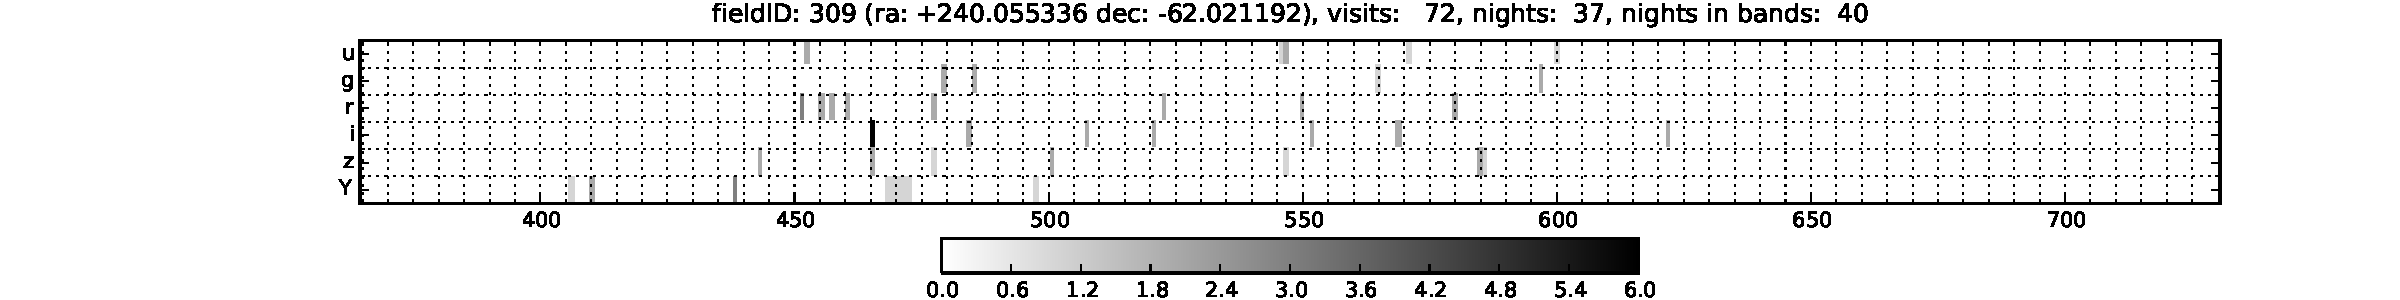
\includegraphics[width=\textwidth]{figs/supernova/fig_309_2ndYear}
 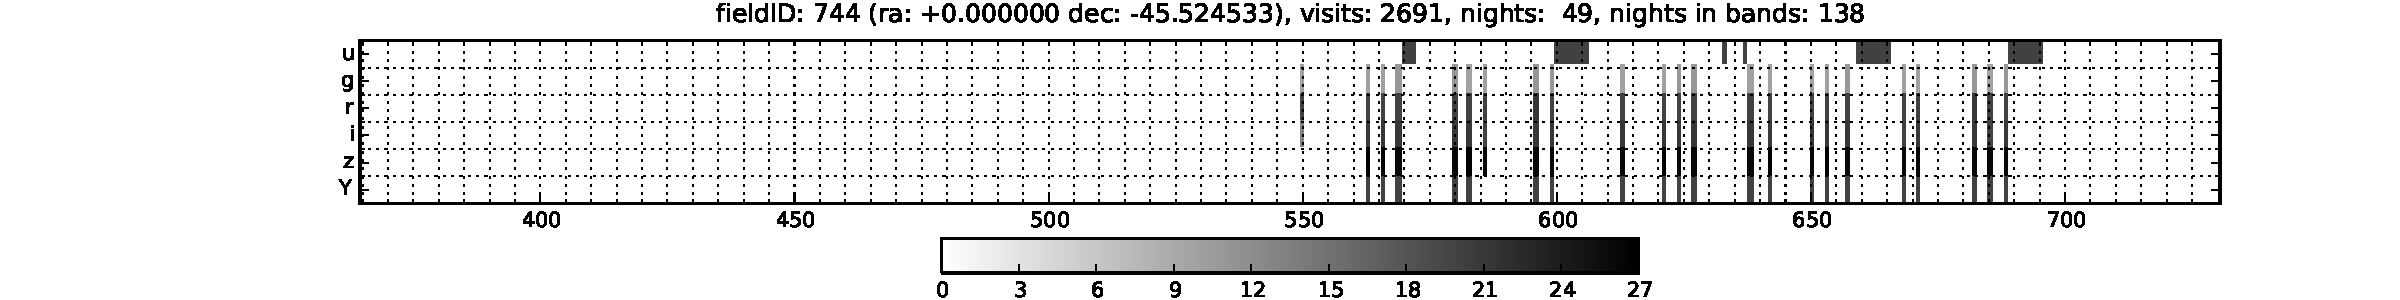
\includegraphics[width=\textwidth]{figs/supernova/fig_744_2ndYear}
 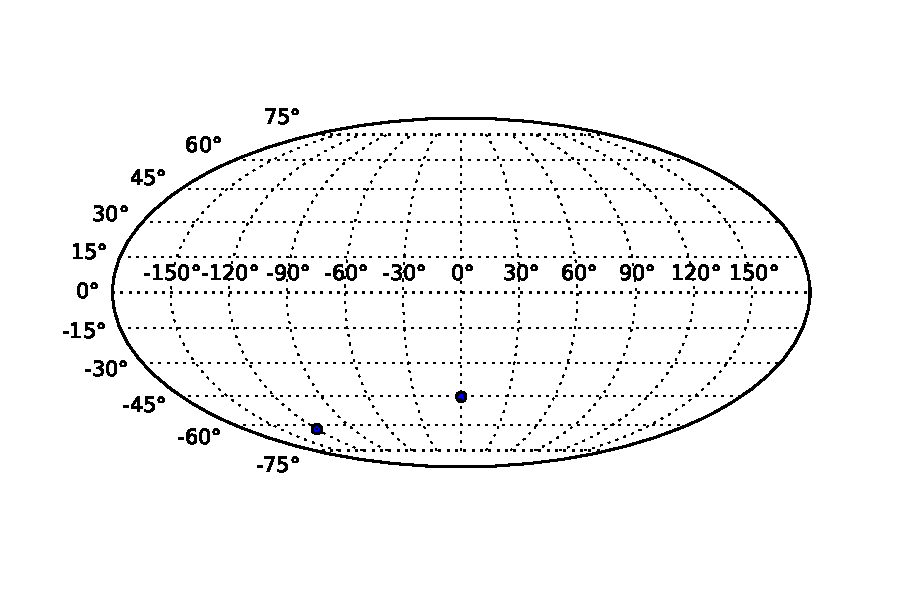
\includegraphics[height=0.2\textheight]{figs/supernova/loc_309_744.pdf}
 \caption{Example of the cadence in the 2nd season in a WFD Field
 (fieldID 309) (top-panel) and a Deep Drilling Field (fieldID 744)
 (middle panel) and the spatial location of these two fields shown on a
 map. The cadence plots show a heatmap of the number of observations per
 night during the second season in each filter u, g, r, i, z, y. 
 The header shows the fieldID and location of
 the field, the total number of visits during that period, the number of
 distinct nights on which observations are taken, and the number of
 distinct observations (where observations are considered indistinct
 if they are on the same night and use the same band).}
  \label{fig:SN_sampling}
\end{figure}


\begin{figure}
\centering
 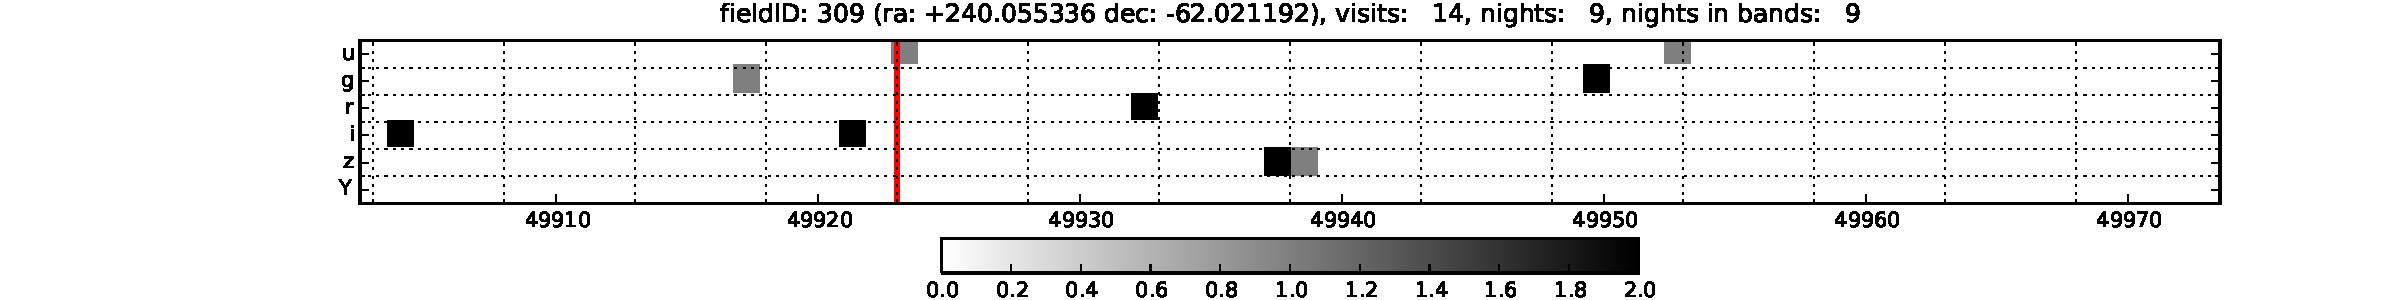
\includegraphics[width=\textwidth]{figs/supernova/TimeWindow_309_49923.pdf}
 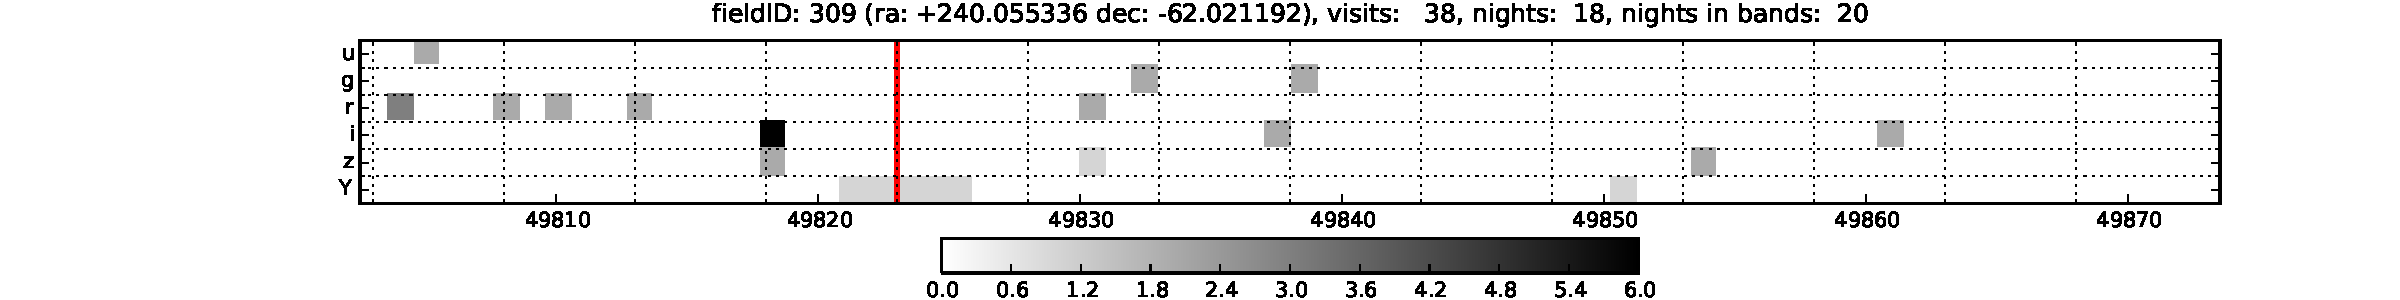
\includegraphics[width=\textwidth]{figs/supernova/TimeWindow_309_49823.pdf}
 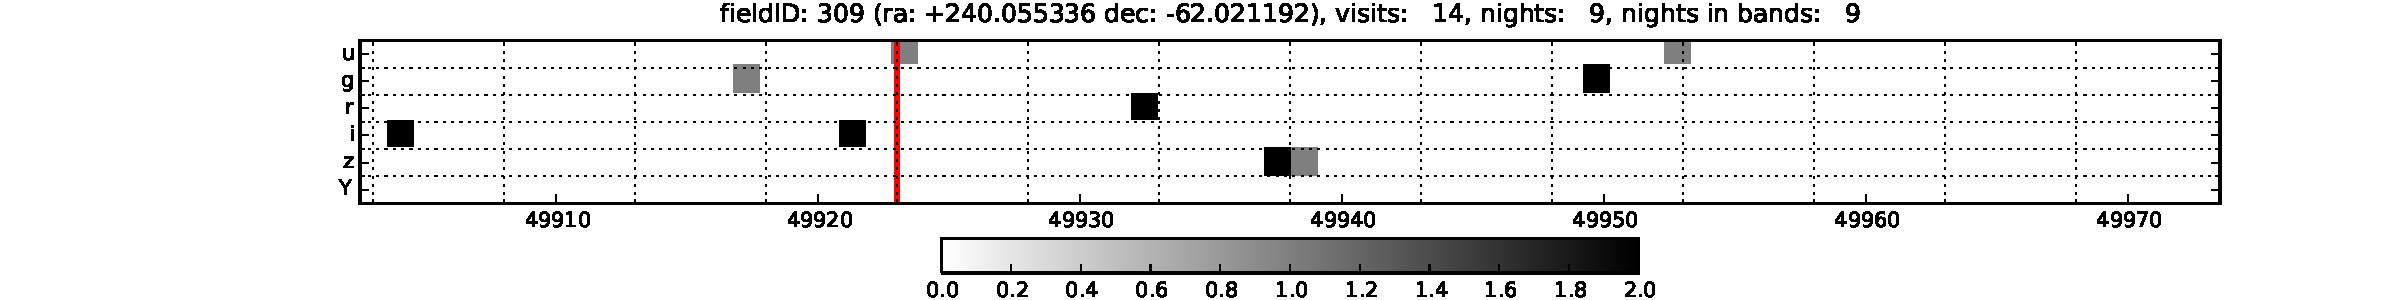
\includegraphics[width=\textwidth]{figs/supernova/TimeWindow_744_49923.pdf}
 %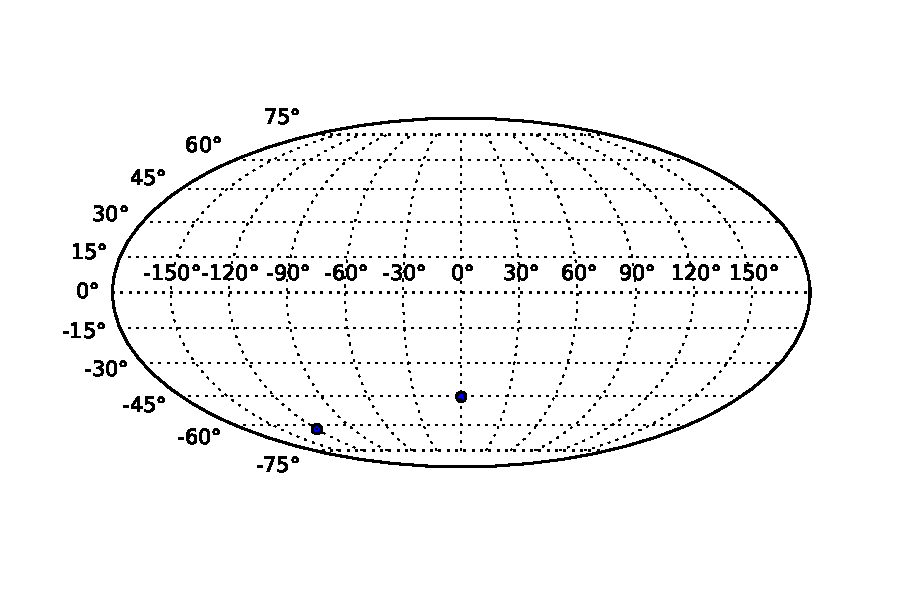
\includegraphics[height=0.2\textheight]{figs/supernova/loc_309_744.pdf}
 \caption{Example of a TimeWindow in a WFD Field (fieldID 309)
 (top-panel) and a second TimeWindow (middle panel) on the same field,
 and a Deep Drilling Field (fieldID 744) (bottom panel) all extending
 -20 days before and 50 days after a chosen night or MJD. For the Deep
 Drilling Field in the bottom panel, and the WFD field in the top
 panel, the chosen date around which the TimeWindow is constructed is
 the MJD of 49923, which is also 570 nights into the survey and marked
 by a red vertical line (which can be used to compare the location to
 \autoref{fig:SN_sampling}. The middle panel shows a window in Field
 309 centered around an MJD of 49823 or a night of 470 which may also be
 compared to \autoref{fig:SN_sampling}. The plots again show the
 heatmap of observations in each filter in each night as in the cadence
 plots of \autoref{fig:SN_sampling}.}
  \label{fig:TimeWindow}
\end{figure}

To define the metric $M,$ we need to define the perSNMetric. Two
different approaches to defining the perSNMetric for a given OpSim run are possible: a) Use
a simulated supernovae Type Ia with specific parameters, observed with
the sequence of observations in the above time-window, and evaluate the
success of each step. b) Study heuristics of the observation sequences by using large simulations 
with randomized parameter values.

Here we will discuss the simpler approach (a). The SN metric in a spatial region
reflects the contribution of the sample of SNe observed in that spatial
region towards inferring the cosmological parameters. Let us
consider a case where each SN observed with conditions better than a
certain threshold contributes equally to the inference. Then the relevant
metric would be a function of the number of SN in the sample passing
such selection criteria. More generally, when the quality of all the
supernovae are not similar, the metric should be thought of as
the weighted sum of supernovae, with the weights being related to the
inverse of the effective variance of the distance modulus:
\begin{equation}
M\sim \sum_i w_i , \qquad  w_i \sim 1.0 /\sigma^2_\mu.
\end{equation}
By comparing with the form of the perSNMetric, we see that the
perSNMetric should be a proxy for $1.0/\sigma^2_\mu,$ where
$\sigma^2_\mu$ is the effective variance on the distance
modulus of the supernova, as determined by fitting an empirical model to the supernova light curve.

%\subsubsection{ Steps in the PerSNMetric}
\subsubsection{Steps in the PerSNMetric}
As described before, the measurement of the distance modulus is the
result of several steps. Therefore, we expect the perSNMetric to be a
product of metrics in each of the steps:

\begin{equation}
PM_i = \prod_{\rm{steps}} PM_i^{\rm{steps}}
\end{equation}

These components of perSNMetric constructed in different steps are
described in \autoref{tab:stepsAndMetrics}.
\begin{center}
 \begin{table}
\begin{tabular}{| p{5cm} |p{10cm}| }
\hline Metric & Description \\
\hline
I. SN discovery  &  Given the observations in a time window corresponding to the lifetime of a supernova, evaluate the  probability of detecting a
transient \\
II. SN classification & Given the observations in a time window corresponding to the lifetime of a 
supernova, evaluate the probability of accurately classifying the transient\\
III. SN light curve characterization quality & Given the observations in a time window corresponding to the lifetime of a supernova, evaluate the quality of characterization\\
\hline 
\end{tabular}
\caption{Components of the perSNMetric}
\label{tab:stepsAndMetrics}
\end{table}
\end{center}



\emph{I. Discovery Metric}

This metric is designed to gauge the performance of detection of SNe 
discussed in \autoref{sec:\secname:targets}.
This metric is a proxy for the probability that a Supernova will be detected
 during its lifetiemby the set of images taken in differnt bands by LSST. A larger
 number of images taken at a time when the supernova is bright enough increases the
 probability of detection. Assuming that a single detection in any of the images containing
 the supernova is sufficient to trigger photometry at the location, one can find the
 probability of detection from a knowledge of SNR-efficiency of detection curve. The Signal to
Noise ratio can be determined given properties of a supernova (redshift, intrinsic brightness etc.)
 and the five sigma depth provided in OpSim. While such a SNR-probability of detection curve does not
 yet exist for the LSST pipeline, one can use such a curve from previous surveys (in particular a
 SNR-efficiency curve constructed during a stage of the Dark Energy Survey for g, r, i, z bands of DES,
 and provided by R. Kessler, priv. communication). This is shown in \autoref{fig:SNR_detection}.
\begin{figure}
 \centering
 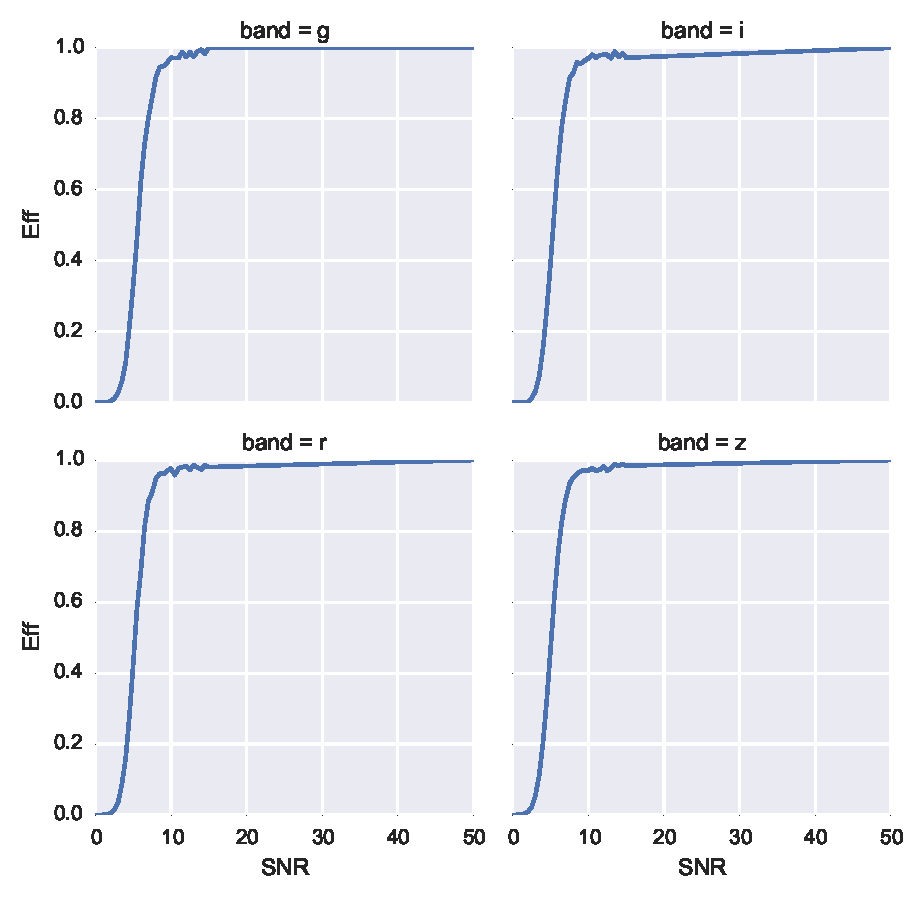
\includegraphics[width=\textwidth]{figs/supernova/SNR_detection.pdf}
 \caption{Probability of detecting a transient from a single Different image in different bands as a
 function of the signal to noise as obtained from Dark Energy Survey, (from R. Kessler). It shows, that 
for high SNR greater than $\sim 10,$ a single exposure used in difference imaging may be sufficient to detect the SN, while for 
lower SNR several such image differences may be necessary to have a high probability of detection.}
 \label{fig:SNR_detection}
\end{figure}





\emph{II. Classification Metric}

Separating supernovae from other detected transients is being considered in 
\autoref{chp:transients}. Here we concern ourselves with problem of classifying subclasses of 
SNe. Multiple techniques have been proposed to solve this problem and it is not yet clear how the 
relative success of these techniques are affected by observing strategy. We thus use the 
multifaceted, machine learning pipeline developed in \citet{Lochner2016} to compare alternative 
observing strategies. The exact metric used to determine the efficacy of the classification depends 
on the exact problem at hand. For producing a general purpose, well-classified set of all types of 
supernovae (for example, to study supernova population statistics), one could use the AUC metric 
defined in \citet{Lochner2016}, which is a good balance between purity and completeness. 
Alternatively, if one only considers supernova cosmology, a simpler metric might be the percentage 
supernova detected if a purity of (for example) 95\% is demanded from the final sample. Work is 
still ongoing to apply the full classification pipeline to multiple OpSim runs and incorporate a 
metric into \texttt{MAF}, combining it with the other components of the perSNMetric.


\emph{III. Quality Metric}

We construct the quality metric for the perSNMetric by obtaining the
light curve of the SN in the time window described above. We fit the
light curve, using the SALT2 model \citep{Guy2007}, and approximately estimate the uncertainty in 
distance from
the light curve fit alone. Of course, as is well known, luminosity
distance estimates of supernova Type Ia also show an intrinsic scatter
of around $0.1$ in previous surveys, which may be expected to decrease
with better training samples and understanding of underlying
correlations of SNIa properties and their environments. We compute a
quality metric for each SNIa as the ratio of the square of the
uncertainty of the distance indicator from the supernova to the square
of the intrinsic dispersion. When added up over SN to obtain a value
$QM$, the uncertainty on cosmological parameters may be expected to
scale as $\sim sqrt(1.0 + \sum QM)$. 

%Move this to OpSim analysis
% The quality metric evaluated on the example SN plotted is $1.0$ if observed in the deep field 
% (\autoref{fig:SNIaLCopsimdeep}), and $0.002$ in the WFD field (\autoref{fig:SNIaLCopsimmain}).



% --------------------------------------------------------------------

\subsection{OpSim Analysis}
\label{sec:\secname:analysis}
The scientific goal of characterizing SNe is to a large extent dependent
on how well the light curves of individual SNe are sampled in time and
filters. To study this, we re-index the OpSim output on spatial
locations rather than use the temporal index. Here we first illustrate
in terms the cadence in two example LSST fields. 

% {\bf Analysis, Results and Discussion}


% \begin{figure}[tbh!]
% %\vskip -1.3in
% 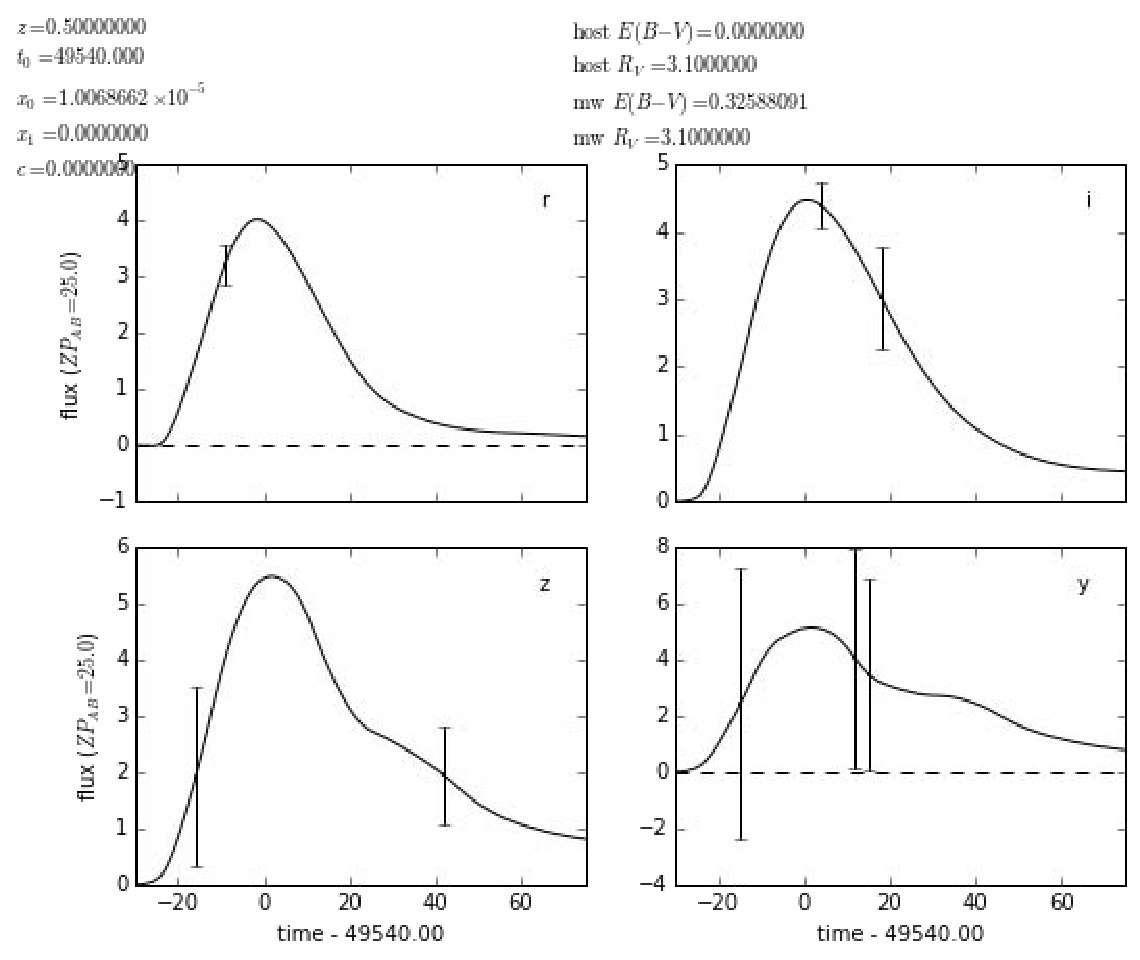
\includegraphics[angle=0,width=0.99\hsize:,clip]{figs/SN_309_lcavg.pdf}
% %\vskip -1.3in
% \caption{Time-interval averaged light curve of
% \autoref{fig:SNIaLCopsimmain}. The light curve shows only a small number
% of the data points, which is insufficient to classify this object as a
% Type Ia and may be also difficult to classify this object as a SN. }
% \label{fig:SNIaLCopsimmain2}
% \end{figure}







% \begin{figure*}[!hb]
%     \begin{minipage}[b]{\linewidth}
%         \includegraphics[width=\textwidth]{figs/supernova/fig_firstSeason_0}
%         \includegraphics[width=\textwidth]{figs/supernova/fig_firstSeason_1}
%         \includegraphics[width=\textwidth]{figs/supernova/fig_firstSeason_2}
%         \includegraphics[width=\textwidth]{figs/supernova/fig_firstSeason_3}
%         \includegraphics[width=\textwidth]{figs/supernova/fig_firstSeason_4}
%     \end{minipage}
% \label{fig:opsimSummary}
% \caption{Cadence of Observations in the timewindow of a year towards a few sample of
% positions. Grey-scale indicates the number of visits. {\it add details}
% }
% \end{figure*}


We analyzed the OpSim output of the Baseline Observing Strategy,
enigma$\_$1189$\_$sqlite.db{\footnote
{\url{http://ops2.tuc.noao.edu/runs/}}} which includes Deep Drilling
Fields (DDF) and the main survey (WFD). Using the OpSim output \texttt{enigma\_1189}, we generated 
light curves for a type Ia supernova with a with a redshift of z=0.5 at a few different
locations. A date in MJD is chosen where the LSST simulated data are
reasonably well populated. We used the SALT2-extended model
with $x_0$, $x_1$ and $c$ set so that the SNIa would have a specific
magnitude of $-19.3$ in the rest frame BessellB band. This was performed
using a version of \texttt{SNCosmo} ~ to interpolate the SALT2 surfaces, and the
LSST catalog simulation package to calculate the flux for LSST
bandpasses. 

%[ML] I'm not sure the number of visits is what's relevant here, multiple visits on a single
%night don't help, except to beat down errors
\autoref{fig:SNIaLCopsimdeep} shows the light curve in
different filters in a deep drilling field. The
number of visits for 50 days (which is the period of the simulated SNIa light curve in
rest-frame, which translates to 75 days at z=0.5) is 53 per filter. For this light
curves, the supernova quality metric (SNQM) and the
discovery metric (SNDM), are both equal to 1. SNDM=1 indicates that this object is a transient that
will be definitely discovered, and SNQM=1 indicates that the light
curves will be of high quality enough to contribute extremely well to
the inference of cosmological parameters. The light curves and
quantified metric demonstrate that data from Deep Drilling Fields would
generate high quality light curves, allowing a high rate of supernova
discovery.

In contrast, \autoref{fig:SNIaLCopsimmain} shows a light curve from the WFD survey. This light 
curve is
generated in Field 290 and has an average number
of data points in the light curve of 2 per filter. Using these light
curves, the probability (SNDM) of detecting this supernova is less
than 0.1. \autoref{fig:perSNCadence} directly compares the light curves and cadences of the two 
fields considered, from the DDF and WFD. 

\begin{figure}
%\vskip -1.3in
%*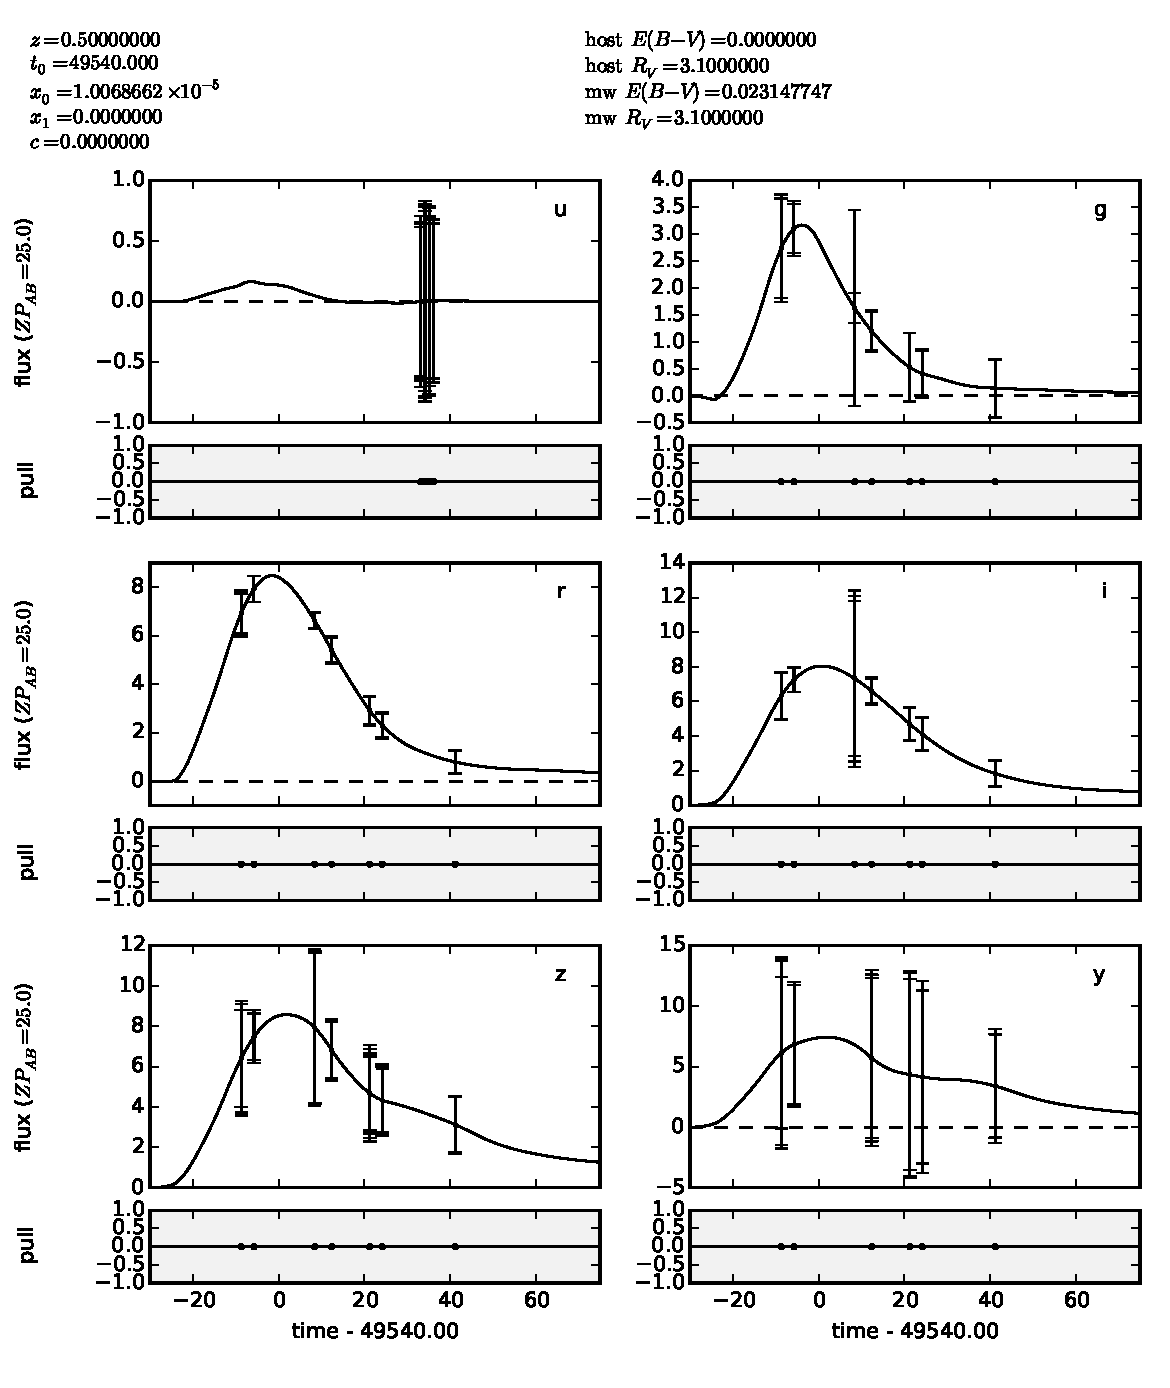
\includegraphics[angle=0,width=0.99\hsize:,clip]{figs/SN_290_lc.pdf}
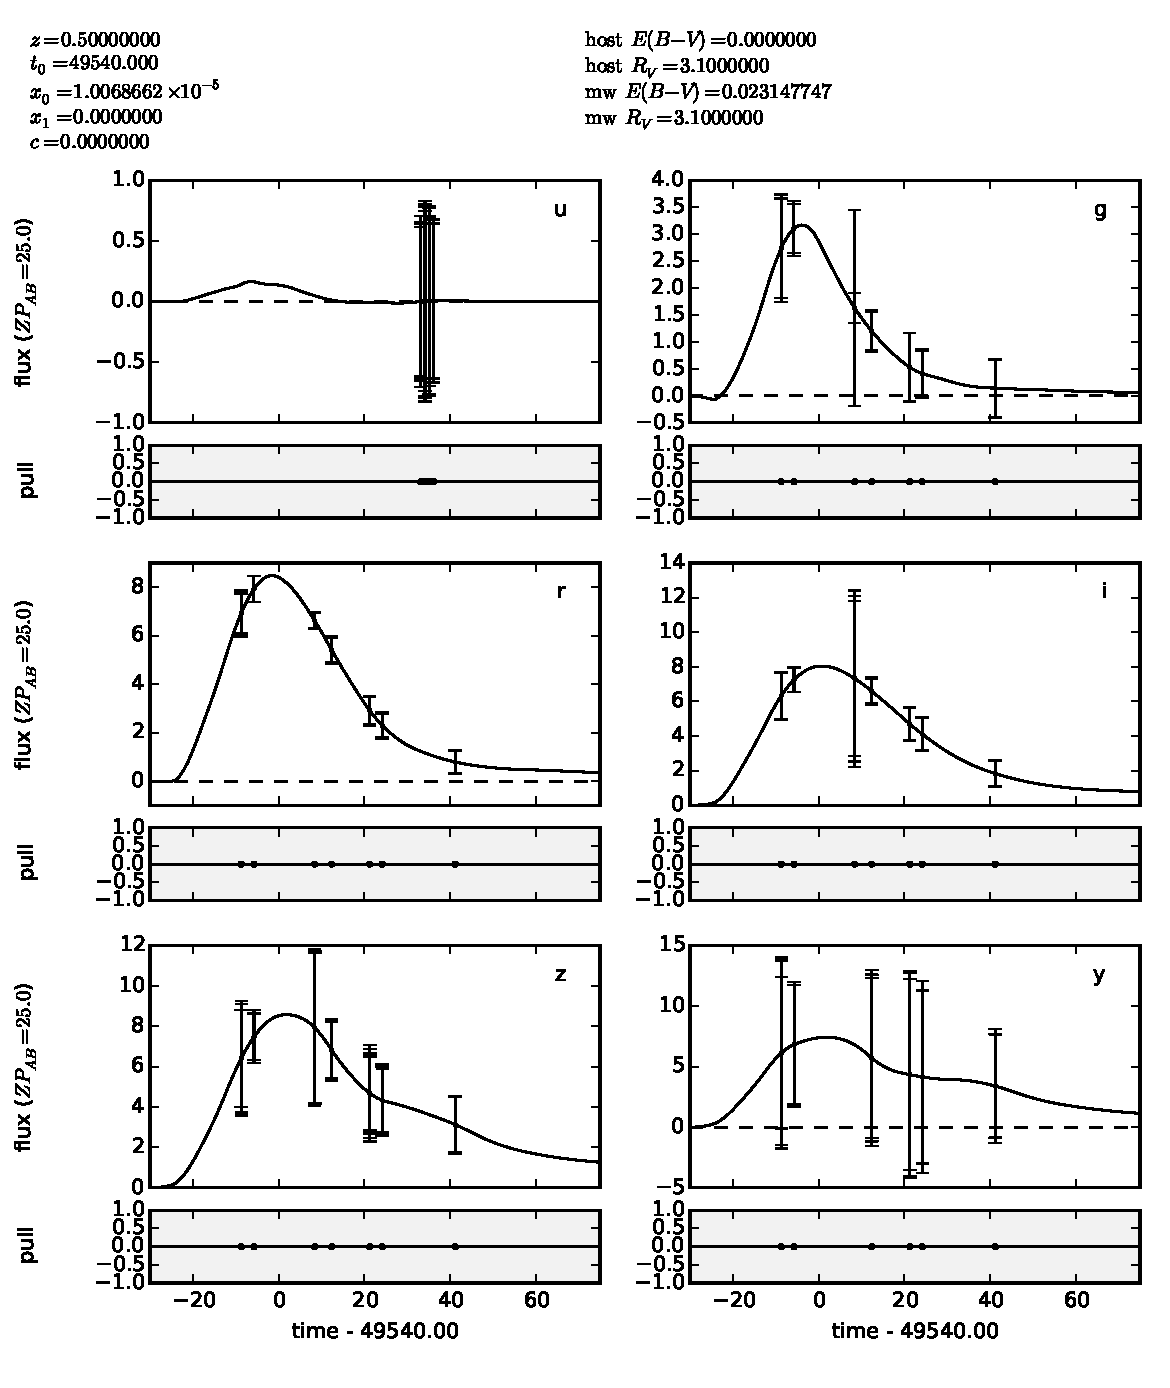
\includegraphics[angle=0,width=14truecm]{figs/SN_290_lc.pdf}
%\vskip -1.3in
\caption{An example of light curve of SN Type Ia using Deep-Drilling
Survey of the LSST Baseline OpSim run.
}
\label{fig:SNIaLCopsimdeep}
\end{figure}

\begin{figure}
%\vskip -1.3in
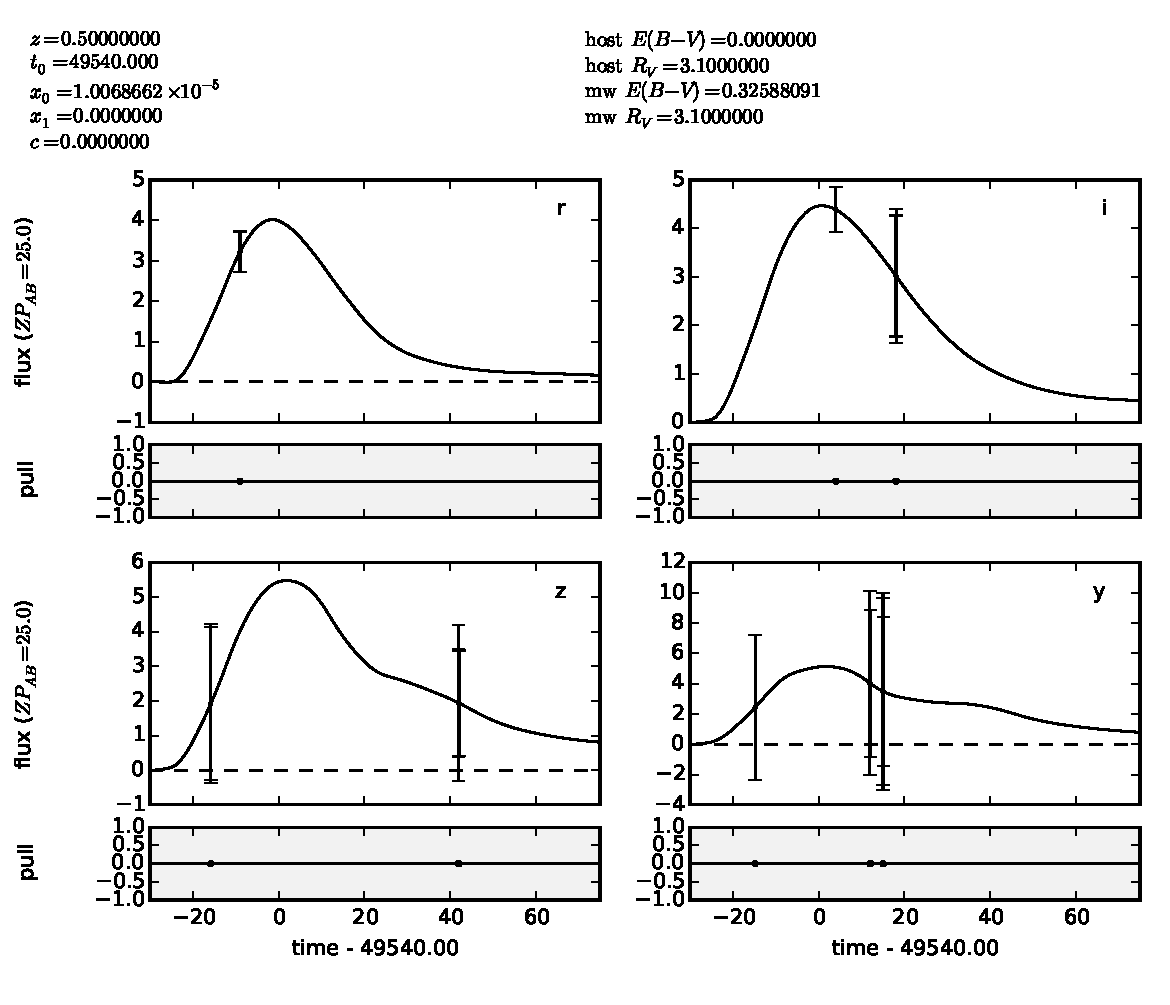
\includegraphics[angle=0,width=0.99\hsize:,clip]{figs/SN_309_lc.pdf}
%\vskip -1.3in
\caption{An example of light curve of SN Type Ia using the Main Survey
of the LSST Baseline \OpSim run.}
\label{fig:SNIaLCopsimmain}
\end{figure}

\begin{figure}
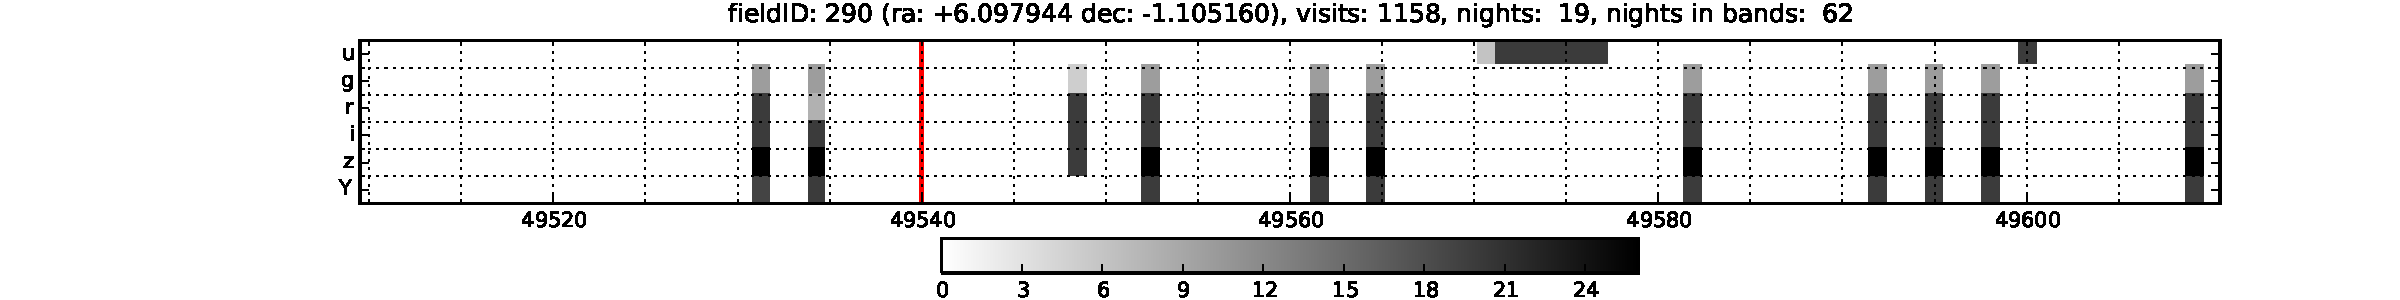
\includegraphics[angle=0,width=\textwidth,clip]{figs/SN_Cadence_290.pdf}
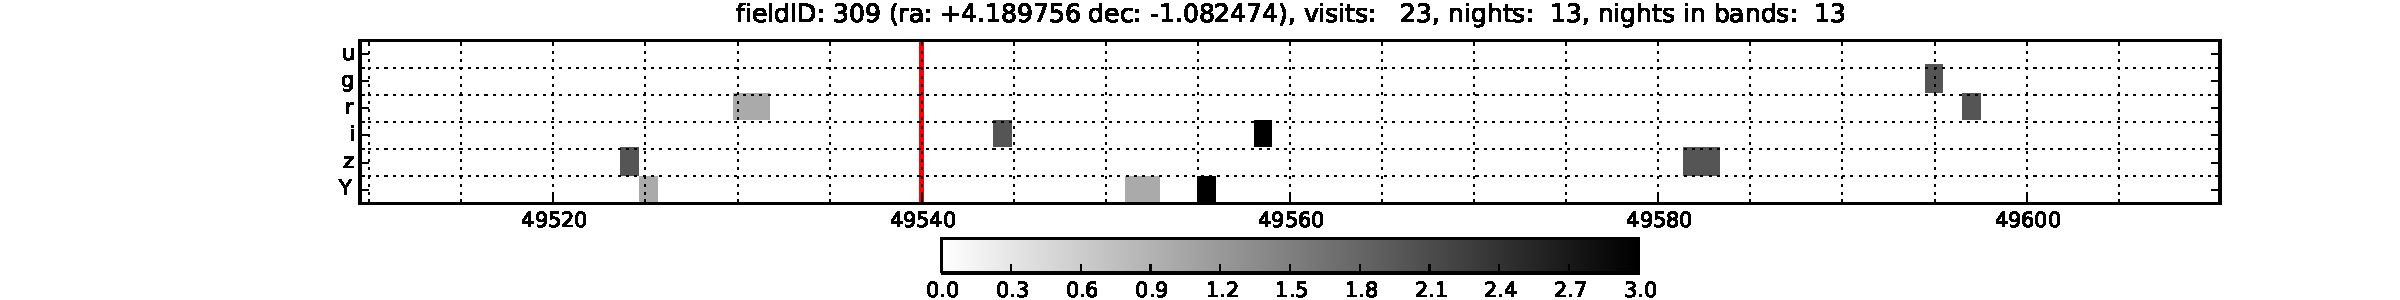
\includegraphics[angle=0,width=\textwidth,clip]{figs/SN_Cadence_309.pdf}
\caption{Cadence of Observations in the timewindow of a representative
supernova at redshift of $z=0.5$ in a DDF (top) field (fieldID: 290) and
a WFD (bottom) field (fieldID: 309). The red lines show the date of
explosion, and the shades show the number of observations in a night in
a distinct filter.}
\label{fig:perSNCadence}
\end{figure}

To further study the quality of light curves across the survey, we simulate the same type Ia 
supernova in 16 different fields, including DDF 290 already studied, from the \texttt{enigma\_1189} 
OpSim run and record the average number of visits per 50 day time window 
(\autoref{tab:lcpositions}). A well-known rule of thumb for good quality SN light curves is to 
demand 7-10 epochs per light curve spread over 50 days or so for more than one filter. Although 
the averages in \autoref{tab:lcpositions} are only approximations because the cadence is 
non-uniform, they give a clear indication that with the \texttt{enigma\_1189} observing strategy, 
the WFD will be largely useless for SNe studies. This motivates our proposal of a rolling cadence 
strategy to improve the sampling of SNe over a much larger area than the DDFs.


% [ML] I've removed this (fairly arbitrary) chategorization, it's more confusing than helpful
% and it's clear how bad WFD is from the numbers alone

% In column 5, we categorize the positions into 5 categories
% base on the data points (the value in column 3) per filter for 50 days.
% When the number of LSST data points (the value in column 3) per filter
% for 50 days is $>$9 as the category A, 5-9 as B, 1.8 -- 5 for C, 1 --
% 1.8 for D, and $<$1 for E. An example of light curve of Category A has
% been shown in Figure \ref{fig:SNIaLCopsimdeep}, Examples light curves of
% Category B have been shown in Figures \ref{fig:SNIaLCopsimmain} and
% \ref{fig:SNIaLCopsimmain2}, respectively. An example of a light curve of
% Category C (ex. Dec.=-40 ;No. 7 in Table \ref{tab:lcpositions}) is shown
% in \autoref{fig:SNIaLCminus40}.

% \new{An example of Category B toward -66$^{\circ}$ is shown
% \autoref{fig:SNIaLCminus66} (No. 3 in \autoref{tab:lcpositions}). The
% light curves in {\it u, g} and {\it r} bands have 3 -- 5 data points,
% while {\it i} band has 8 or more than data points. The band z and y show
% relatively large error bars. In order to increase probability to
% recognize the light curve as a SN and Type Ia, simulated LSST data
% points could be increased by a factor of 2-3. Our goal is to improve the
% light curves which belong to Category B and C so that we can distinguish
% them as a SN and particularly as a Type Ia SN. This will improve values
% in SNDM and SNQM.}

\begin{center}
\begin{table}
%\tabletypesize{\scriptsize}
\centering
\begin{tabular}{|p{0.9cm} |p{3.3cm}|p{4cm}|p{1.7cm}|}
\hline
 Field or No. & (RA,Dec) & No. of LSST visits per year (u,g,r,i,z,y)       & Avg. No.\\
\hline
290 DDF  & (349.386,-63.321)  & 2363 (398,229,402,414, 522,396) & 53 \\
 1      & (190,-83) &    239 (38,41,41,44,33,42) & 5.3\\
 2      &(20,-83) & 252 (52,56,40,21,37,44)  &5.7\\
%old 3      &(120.012,-71.879) &  220(36,38,37,32,44,33) & 5.0 & B &\\
3      &(116,-66) &  220 (36,38,37,32,44,33) & 5.0  \\
 4      &(240.05,-62.02) &101 (2,5,11,19,19,45) & 2.2  \\
 5      &(120,-50)  &80 (4,7,9,18,24,18)        & 1.8\\
 6      & (80,-40)  &      96 (5,8,15,17,27,24) &  2.2\\
 7      & (280,-40) &      86 (4,2,6,4,24,18)   &  2.0\\
 8      & (30,-20)  &      86 (3,4,10,21,27,21) &  1.96\\
 9      & (100,-20) &      58 (4,2,6,4,24,18)   &  1.3\\
% 000  & (358.41,+0.18)  &                      &     & C({\it 0.1}) & \ref{fig:SNIaLCDecp18}\\
 309  & (6.097, -1.105) & 80 (4,7,9,18,24,18)  & 1.83\\
% 290  & (6.097, -1.105) &                      &     & C({\it 0.1}) & \ref{fig:SNIaLCDecp18}\\
 11     & (50,+1.5) &      72 (3,6,10,12,22,19) &  1.64\\
 12     & (320, +5) &      7 (0,0,2,0,4,0)      &  0.15\\
 13     & (60,+5)   &      66 (0,7,11,20,28,0)  &  1.5 \\
 14     & (60,+20)  &      72 (0,8,13,22,29,0)  &  1.64\\
 15     & (60,+30)  &      44 (0,5,6,15,18,0)   &  1.0\\
\hline
\end{tabular}
\caption{Table of 16 fields in the OpSim \texttt{enigma\_1189}. The first column is simply an 
index, with the special example fields of the DDF field 290 and WFD field 309 indicated. The 
position of the fields is shown in column 2. The third column contains the total and per filter 
band number of visits per year and this is averaged per filter per 50 day time window in column 4. 
It can be seen that with this observing strategy, only the deep drilling fields are suitable for 
supernova cosmology, where 7-9 data points per filter band is considered adequate quality.}
\label{tab:lcpositions}
\end{table}
\end{center}

% \begin{center}
% \begin{table}
% %\tabletypesize{\scriptsize}
% \begin{tabular}{|p{0.7cm} |p{2.8cm}|p{4cm}|p{1.7cm}|p{1.4cm}|p{0.7cm}|}
% \hline
%  Field or No. & (RA,Dec) & No. of LSST data per year (u,g,r,i,z,y)       & Avg. No.&Category (TPR) 
% &Fig. No. \\
% % Field or [No.] & (RA,Dec) & No. of LSST data per year (u,g,r,i,z,y)       & Avg. No. per filter 
% per 50 days   &Category (TPR)\\
% %  or No.      &  (J2000)  & per year (u,g,r,i,z,y) & per filter & (TPR)    \\
% %        &           &                        & per 50days &     \\
% 290 DDF  & (349.386,-63.321)  & 2363(398,229,402,414, 522,396) & 53 & 
% A(1)&\ref{fig:SNIaLCopsimdeep} 
%  \\
%  1      & (190,-83) &    239(38,41,41,44,33,42) & 5.3 & B ({\it 0.4}) & \\
%  2      &(20,-83) & 252(52,56,40,21,37,44)  &5.7  & B  & \\
% %old 3      &(120.012,-71.879) &  220(36,38,37,32,44,33) & 5.0 & B &\\
% 3      &(116,-66) &  {\it 220(36,38,37,32,44,33)} & 5.0 & B & \ref{fig:SNIaLCminus66} \\
%  4      &(240.05,-62.02) &101(2,5,11,19,19,45) & 2.2  & B & \ref{fig:SNIaLCopsimmain2}\\
%  5      &(120,-50)  &80(4,7,9,18,24,18)        & 1.8 &  C &\\
%  6      & (80,-40)  &      96(5,8,15,17,27,24) &  2.2 & C &\\
%  7      & (280,-40) &      86(4,2,6,4,24,18)   &  2.0& C &\\
%  8      & (30,-20)  &      86(3,4,10,21,27,21) &  1.96& C & \\
%  9      & (100,-20) &      58(4,2,6,4,24,18)   &  1.3& D &\\
% % 000  & (358.41,+0.18)  &                      &     & C({\it 0.1}) & \ref{fig:SNIaLCDecp18}\\
%  309  & (6.097, -1.105) & 80 (4,7,9,18,24,18)  & 1.83   & C({\it 0.1}) & \ref{fig:SNIaLCDecp18}\\
% % 290  & (6.097, -1.105) &                      &     & C({\it 0.1}) & \ref{fig:SNIaLCDecp18}\\
%  11     & (50,+1.5) &      72(3,6,10,12,22,19) &  1.64& D &\\
%  12     & (320, +5) &      7(0,0,2,0,4,0)      &  0.15& E &\\
%  13     & (60,+5)   &      66(0,7,11,20,28,0)  &  1.5  & D& \\
%  14     & (60,+20)  &      72(0,8,13,22,29,0)  &  1.64& D &\\
%  15     & (60,+30)  &      44(0,5,6,15,18,0)   &  1.0& E &\\
% \hline
% \end{tabular}
% \label{tab:lcpositions}
% \end{table}
% \end{center}


% \emph{To be added: 2 more examples of light curves at different positions of sky.}

% \begin{figure}[tbh!]
% %\vskip -1.3in
% 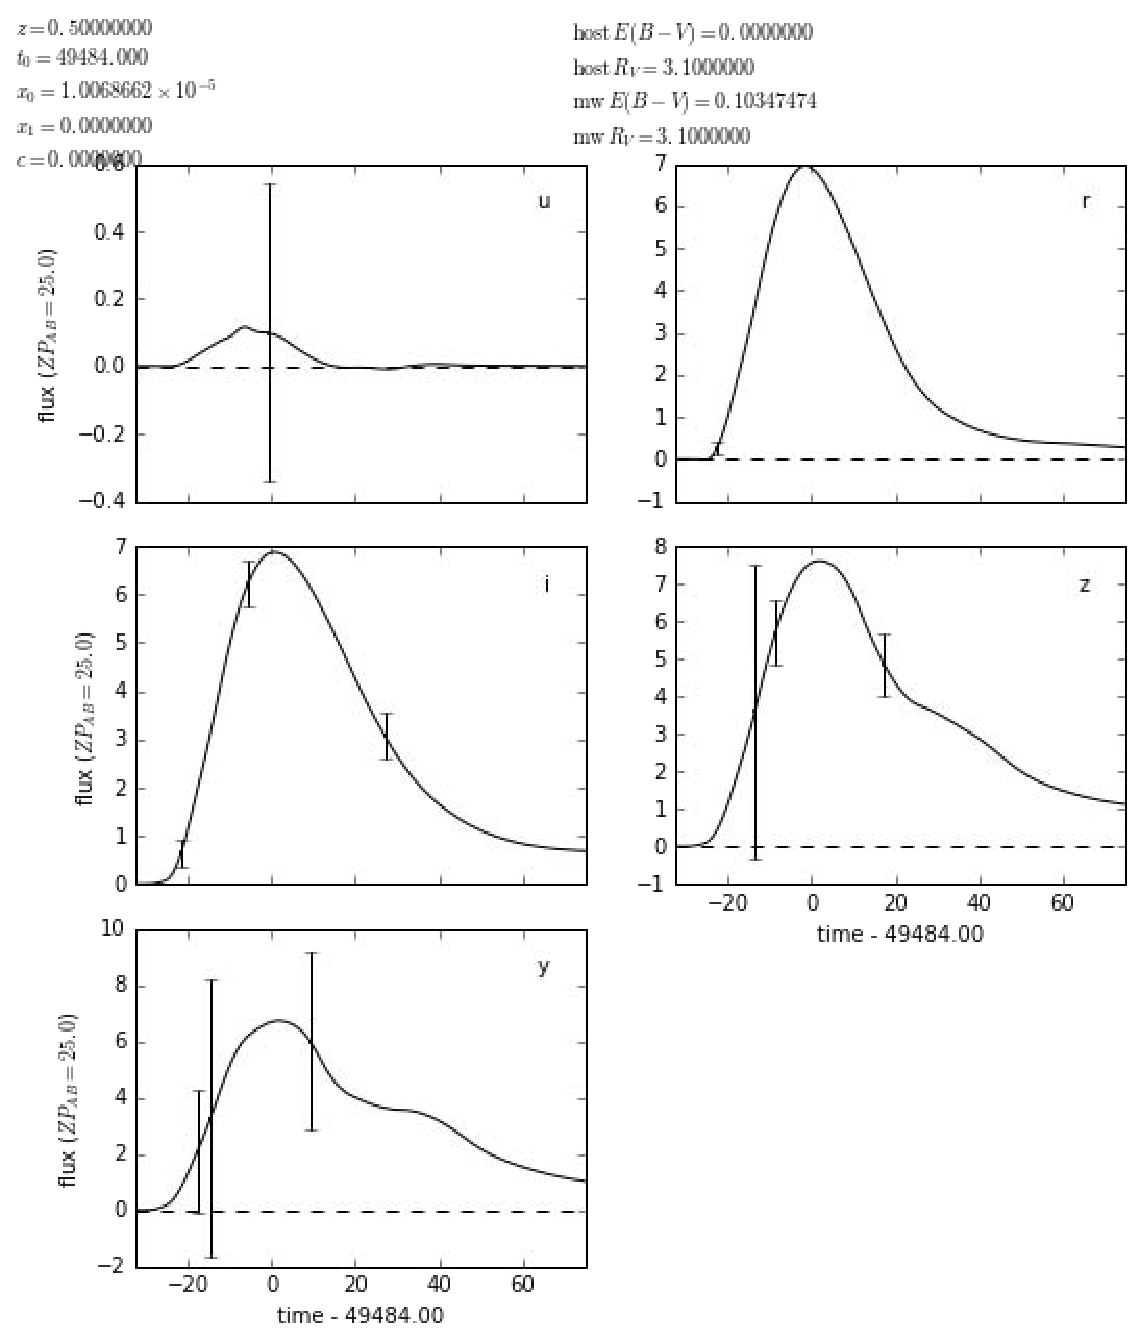
\includegraphics[angle=0,width=0.99\hsize:,clip]{figs/supernova/LCDecminus40no40.pdf}
% %\vskip -1.3in
% \caption{An example of light curve of SN Type Ia (Dec. of -40$^{\circ}$: No. 6) using
% the Main Survey of the LSST Baseline OpSim run. }
% \label{fig:SNIaLCminus40}
% \end{figure}
% 
% \begin{figure}[tbh!]
% %\vskip -1.3in
% 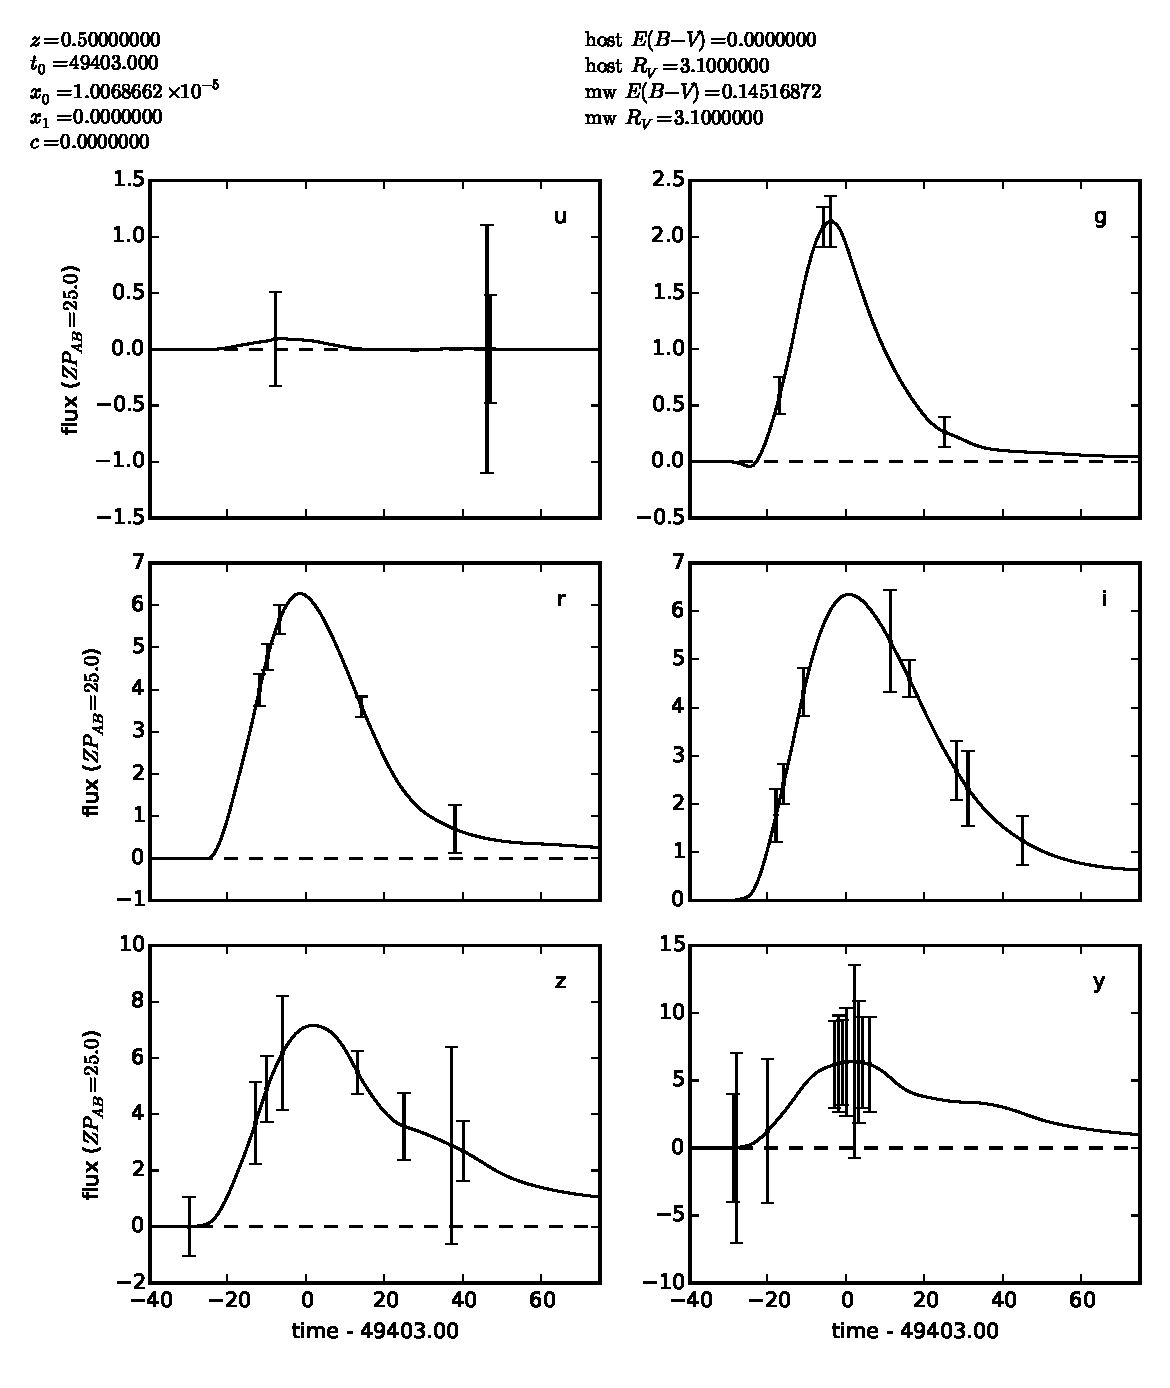
\includegraphics[angle=0,width=0.99\hsize:,clip]{figs/supernova/s1_lc_coaddedDecminus66RA115.pdf}
% %\vskip -1.3in
% \caption{An example of light curve of Type Ia in the direction to Dec. of -66$^{\circ}$
%  using the Main Survey of the LSST Baseline OpSim run.
% }
% \label{fig:SNIaLCminus66}
% \end{figure}
% 
% 
% \begin{figure}[tbh!]
% %\vskip -1.3in
% 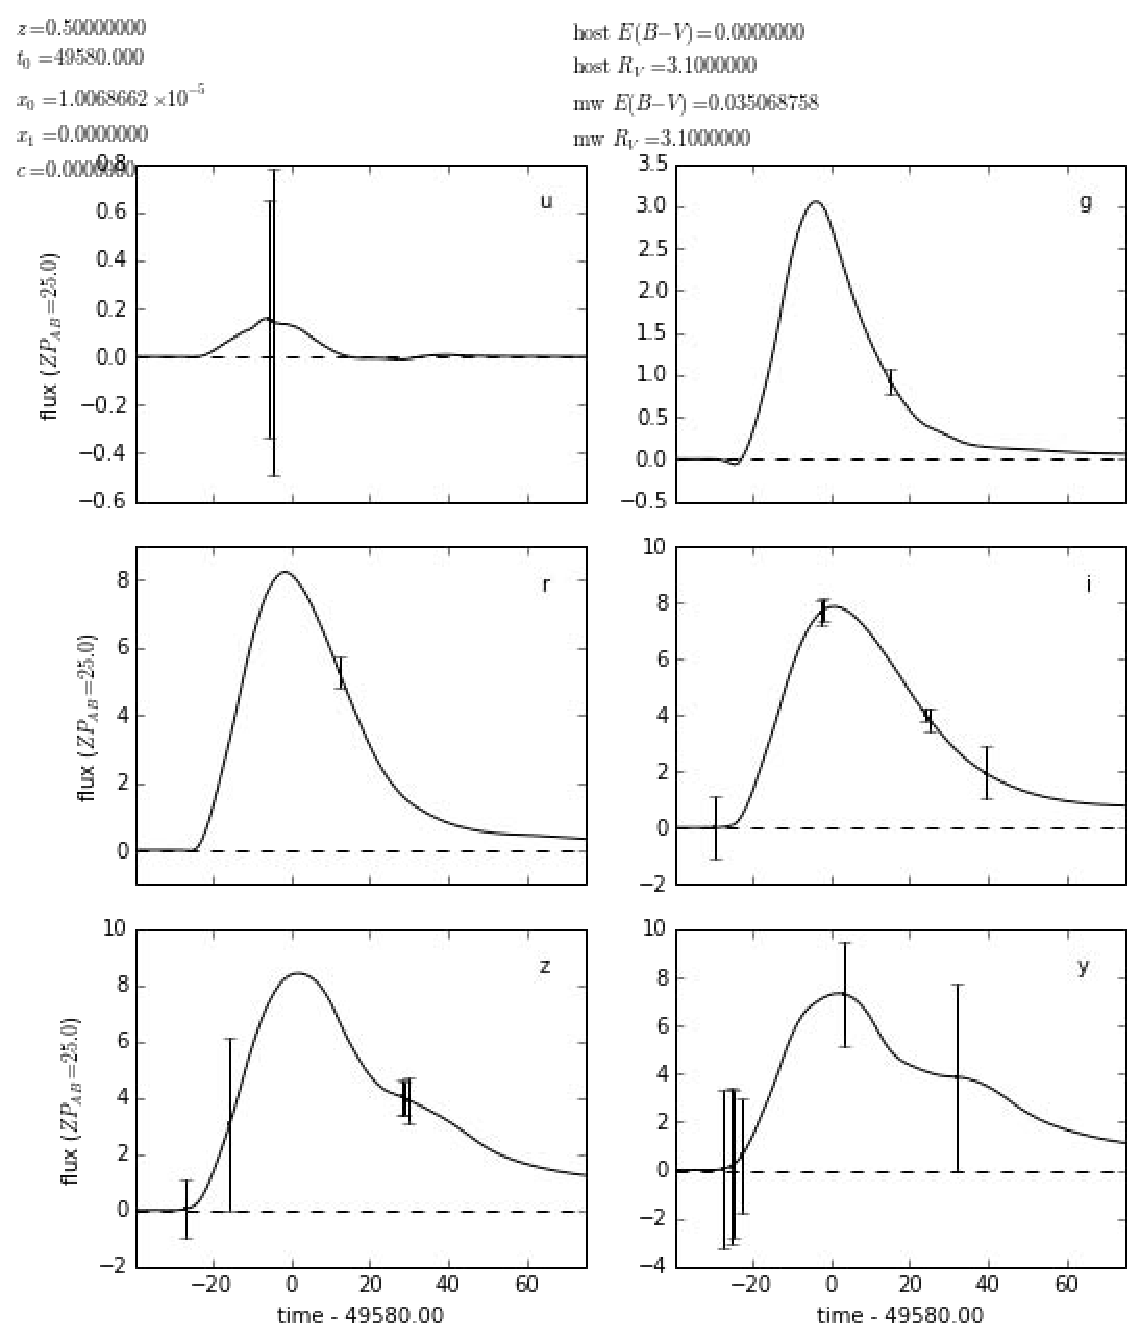
\includegraphics[angle=0,width=0.99\hsize:,clip]{figs/supernova/LCfield00Decp18RA358.pdf}
% %\vskip -1.3i
% \caption{}
% %\caption{An example of light curve of Type Ia in the direction (RA, Dec.)=(358.41, +0.18)
% % using the Main Survey of the LSST Baseline OpSim run. A representative lightcurve
% % of Category C.
% %}
% \label{fig:SNIaLCDecp18}
% \end{figure}



% --------------------------------------------------------------------

\subsection{Discussion}
For the current baseline observing strategy, the DDF fields will produce an exquisite sample of 
well-characterized SNe for cosmology and astrophysics studies. Further analysis is required to 
determine exactly how many (useful) supernovae will be detected and what the resulting cosmological 
constraints will be, but in this section we have discussed and motivated several important 
intermediate metrics.

\subsubsection{Scientific Motivation for Rolling Cadence}
It is clear from the above analysis, that the WFD component of the LSST survey will not be useful 
for supernova cosmology. However, with some changes to the observing strategy, it is likely that a 
large part of the WFD can be leveraged by implementing a rolling cadence strategy. The idea is to 
sample a particular field with much higher cadence, at the expense of other fields, for a period of 
time (such as 50-100 days) and change fields throughout the survey to preserve uniformity by the end 
of the 10 year period. Ideally, we would propose changing the filter every day, and trebling the 
average WFD cadence in these smaller fields. This would achieve our goal of 7-9 points per light 
curve over a 50 day period and in addition, the variety of filters would result in extremely 
well-characterized SNe in several bands that will thus be also be more easily classified.  

% \subsection{Rolling Cadence of the Main Survey Optimized for Supernova Science}
% 
% \subsubsection{ Scientific Motivation for Rolling-Cadence}
% 
% The main survey is important for the discovery of supernovae (SNe) in
% the redshift range of 0.1- 1, which is critical to constraint SN
% cosmological parameters. In order to identify a variable source as a SN
% and to distinguish the source as a Type Ia SN, we need 7-10 epochs
% spread over 45 days or so for each filter based on past experience.
% Universal survey of the Baseline Cadence provides 6 filter data for
% approximately 18 days (assuming a survey with a filter can be done for 3
% days). This provides 15 data points over 45 days and 2.5 data points in
% average for each filter. Our analysis of OpSim run (Baseline Observing
% Strategy) output shows the light curves of SNe from the OpSim data are
% insufficient not only to identify the source as a SN and but also to
% classify the SN if the SN is type Ia or II (or Ib, Ic). Our proposed
% observing strategy is critical to improve the quality of SN light
% curves. The light curves will have at least 3 times densely populated
% data points in time.
% 
% 
% \subsubsection{Proposed Rolling-Cadence of the Main Survey Optimized for SN Science }
%\label{sec:\secname:discussion}

% {\it Discussion: what risks have been identified? What suggestions could be
% made to improve this science project's figure of merit, and mitigate
% the identified risks?}
% 
% Our goal for observing strategy optimized for SN cosmology is to
% obtain 7-10 epochs spread over 50 days or so for more than one filter. We suggest to
% change the filter every day and LSST can choose a part of sky which has the best airmass,
% centered on Zenith. LSST will observe about 1/3 of visible sky per day (to be confirmed).
% LSST can observe the same part of sky for 6 days with 6 filters, and repeat 9 times for
% the same field. This observing strategy will result in 54 visits (with 6 different
% filters) for the same field. We repeat the same for Field 2 which takes another 54 days.
% Then observe Field 3 for another 54 days.
% 
% We propose a new Observing Strategy of the main survey (the Universal Cadence area;
% WFD) in order to generate 3 times densely populated SN light curves in time (i.e. 3
% times higher samples for a SN light curve). Our main goal is to obtain 7-10 epochs
% spread over 45 days per filter. For simplicity, we assume the main survey will cover
% available sky (2293 fields) for 3 days (we divide the available sky into 3 separate
% Sectors, which would be called Sector 1 and 2 and 3. Each Sector of the sky
% corresponds to ~764 fields. The sum of Sector 1 and 2 and 3 is 2293 fields, a total
% number of LSST fields from the Universal Cadence area. For a day, 1/3 of available
% sky would be observed. By changing the filter, every day, it will take 6 days to
% observe 6 filters for 1/3 of available sky. We repeat 9 times for the same Sector of
% sky, which will result in 54 visits (with 6 different filters) for the same Sector
% (1/3 of available sky). We repeat the same for the 2nd Sector of sky which takes
% another 54 days. Then we observe the 3rd Sector for another 54 days.
% 
% To visualize this idea, we list our proposed observing strategy day by day; Day 1 :
% Filter 1 (for the 1st Sector), Day 2: Filter 2 (for the 1st Sector), Day 3: Filter 3
% (for the 1st Sector), Day 4: Filter 4 (for the 1st Sector), Day 5: Filter 5 (for the
% 1st Sector), and Day 6: Filter 6 (for the 1st Sector). Repeat this sequence 9 times
% for the 1st Sector. This will generate 54 data points for 54 days for a supernova and
% 9 data points in average for each filter. This is approximately 3 times higher sample
% of data for 54 days than those from the Universal Cadence. Observe the same sequences
% for the 2nd Sector (it takes 54 days) and then do the same for the 3rd Sector of sky
% (it takes another 54 days). This summarizes overall idea, but since visible sky is
% slightly different every day and observation depends on the weather, an OpSim run is
% needed accounting for all of these factors (and maybe other factors that we haven't
% mentioned here). One may also consider to observe each Sector for 108 days (2x54
% days) instead of 54 days; this may allow us to discover a higher number of SNe in
% stead of for 54 days. Our suggestion is mainly for the sky of Galactic latitude
% greater than 30 degree (|l| > 30) since it would be hard to discover SNe at the
% Galactic plane.
% 
% \subsubsection{Expectations}
% 
% \begin{enumerate}
% \item SN light curves would have 3 times more densely populated in time as we have designed.
% \item An average airmass of the Main Survey would be significantly lower.
% \item Significantly higher number of SN discovery can be expected because its impact area is
% large. The average number of visits per filter for 50 days is only $\sim$2 for the regions
% located from Dec. -65 to Dec. 0 based on Baseline Observing Strategy, but the number would
% be $\sim$6 with our proposed rolling cadence.
% \end{enumerate}



% %\begin{figure}[tbh!]
% \begin{figure}
% \vskip 3truecm
% %\vskip -1.3in
% %\includegraphics[angle=0,width=0.99\hsize:,clip]{figs/SNIaLCopsim.pdf}
% %\vskip -1.3in
% \caption{Predicted light curves of Supernova Type Ia using
% Rolling-Cadence. We used ramdom generation of time sequence (TO BE
% INCLUDED).}
% \label{fig:SNIaLCopsimmainnew}
% \end{figure}



% \begin{itemize}
% \item Intrinsic Dispersion, environmental effects, newer analysis methods
% \item Follow-up
% procedures: What is feasible? Where will our training samples for classification and light
% curve models come from (other experiments, our own sub-samples with spectroscopic
% follow-up?), spectroscopic follow-up of host galaxies. Can hosts be identified?
% \item `Systematics': In what ways will the real data not match the assumptions made in analysis.
% Having a large sample of SN, to understand the astrophysics would be useful for this.
% \end{itemize}


% ====================================================================

\navigationbar

%\end{document}
